\documentclass[conference]{IEEEtran}
\IEEEoverridecommandlockouts
% The preceding line is only needed to identify funding in the first footnote. If that is unneeded, please comment it out.

\usepackage{cite}
\usepackage{amsmath,amssymb,amsfonts}
\usepackage{algorithmic}
\usepackage{graphicx}
\usepackage{textcomp}
\usepackage{hhline}
\usepackage{subcaption}
\usepackage{threeparttable}
\usepackage{comment}
%\usepackage{xcolor}
\usepackage[table]{xcolor}
\usepackage{float}
\usepackage{multicol}
\usepackage{listings}
\usepackage{xparse}
\usepackage{gvv}

\def\BibTeX{{\rm B\kern-.05em{\sc i\kern-.025em b}\kern-.08em
    T\kern-.1667em\lower.7ex\hbox{E}\kern-.125emX}}
\begin{document}

\title{Implementation of Open Source Software NavIC L1 Transmitter and Receiver\\
}

\author{\IEEEauthorblockN{Satheesh Kumar Simhachalam}
\IEEEauthorblockA{\textit{PhD Scholar} \\
\textit{EE Department, IIT Hyderabad}\\
Telangana, India - 502284 \\
gadepall@ee.iith.ac.in}
\and
\IEEEauthorblockN{ Dr G.V.V.Sharma}
\IEEEauthorblockA{\textit{Associate Professor} \\
\textit{EE Department, IIT Hyderabad}\\
Telangana, India - 502284 \\
gadepall@ee.iith.ac.in}
\and
\IEEEauthorblockN{ Dr. Kuchi Kiran Kumar}
\IEEEauthorblockA{\textit{Professor} \\
\textit{EE Department, IIT Hyderabad}\\
Telangana, India - 502284 \\
kkuchi@ee.iith.ac.in}

}

\maketitle

\begin{abstract}
This paper presents an open source software implementation of NavIC L1 transmitter and receiver for SPS singal used for civilian purposes. 
It describes signal chacteristics, various singal processing blocks of both transmitter \& receiver and channel modelling details. Simulation results 
are presented using random Navigation data genereated at transmitter end and verifying the same at receiver end.
\end{abstract}

\begin{IEEEkeywords}
NavIC, SPS singal, BCH, LDPC, BOC signal, Navigation (NAV) message, Acquisition, Tracking, Encoder, Decoder, Demodulator
\end{IEEEkeywords}

\section{Introduction}
NavIC is an independent regional navigation satellite system developed and maintained by Indian Space Research 
Organisation (ISRO). 
It provides accurate position and timing services to users in India as well as the region extending
upto 1500 km from its boundary. NavIC provides two types of services, namely, Standard Positioning 
Service (SPS) and Restricted Service (RS) with a position accuracy of better than 20m over the 
primary service area and timing accuracy better than 50ns.  

The current NavIC satellite constellation comprises of six operational navigation satellites, 
out of which one satellite has civilian L1 band (1575.42 MHz) transponder providing SPS service 
for low power receivers. ISRO has plans to launch more satellites with L1 band, in future. 
SPS signals from NavIC are interoperable with other GNSS systems like GPS and GLONASS etc. 

The Government of India mandated all mobile device manufatures to have support for navigation 
using NavIC in all the devices being used in India. Hence, there is a growing need for NavIC 
software implementations. \cite{b1} describes open source software implementation for Galileo signal,
however, for Navic L1, no such implementation was found in the literature survey. So, this paper 
focuses on building an open source software implementation of Navic L1 transmitter 
(to simulate Navic L1 signal) and NavIC L1 receiver for SPS services. 

The scope of implementation (done in Python) is limited to generating an SPS baseband signal,
sending baseband signal (without a carrier) thorugh transmitter module, mixing it with channel 
modelling module and verifying that the same navigations bits are received at the output of the 
receiver module. 

\section{System Overview}
The block diagram of the system is shown in Figure \ref{fig:sim_flow}. Navigation data is randomly 
generated and subframes $\&$ master frames are created as per the frame structure described in 
subsequent sections. The transmitter module creates the required baseband signal as per the  
modulation scheme, with relevant channel encoding schemes and error correction $\&$ detection schemes. 
Channel modelling module adds various modelling parameters and AWGN noise to the baseband signals 
for different satellites, forming a composite signal. The receiver module receives the composite 
signal, processes it to extract the navigation data, that was originally sent.   


\begin{figure}[ht] 
\centering
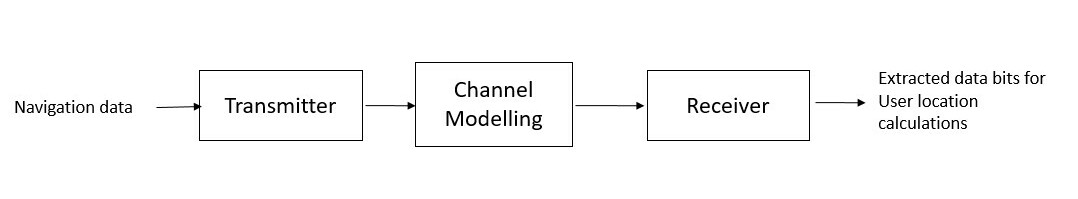
\includegraphics[width=1\columnwidth]{figs/simulation_overview.jpg}
\centering
\caption{System Overview}
\label{fig:sim_flow}
\end{figure}

\section{Software Implementation of Transmitter}
The NavIC transmitter is simulated to send baseband signal to the channel as shown in Fig \ref{fig:trans_flow}.

\begin{figure}[ht]
    \centering
    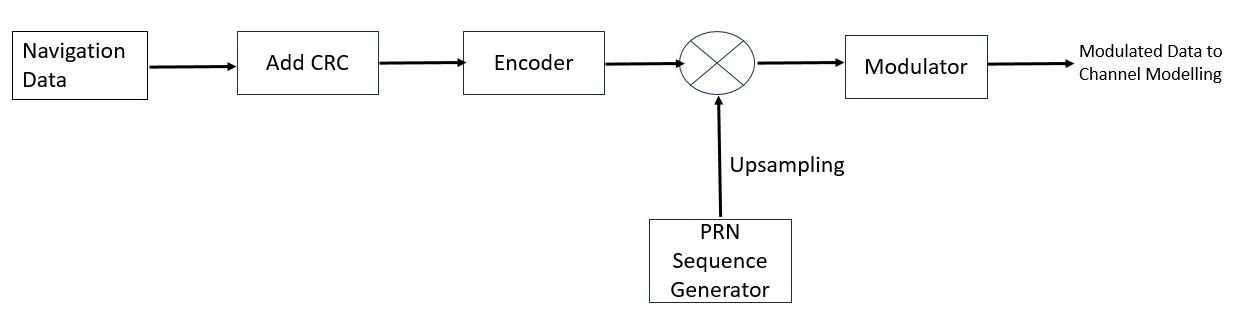
\includegraphics[width=1\columnwidth]{figs/trans_flow.jpg}
    \centering
    \caption{Transmitter Block diagram}
    \label{fig:trans_flow}
    \end{figure}


\subsection{Modulation Scheme} \label{AA} 
The SPS signal is modulated using Synthesized Binary Offset Carrier (SBOC) modulation 
scheme \cite{b2}, comprising of data signal and pilot signal. Both these signals 
contain BOC(1,1) and BOC(6,1) components. In this modulation scheme, data channel BOC(6,1) 
component is generated by interplexing data channel BOC(1,1), pilot channel BOC(1,1) and pilot 
channel BOC(6,1) components. Subsequently, the data and the pilot signals are quadrature 
multiplexed with each other with power sharing of 41.82$\%$ and 58.18$\%$, respectively for each 
of the signals to provide the constant envelope modulation. 

\subsubsection{Mathematical Equations}
\noindent The mathematical representation \cite{b1},\cite{b2} of baseband navigation signals is as follows:

\noindent\textbf{Pilot Signal:}
\begin{multline}
S_{p,a}(t) = \sum_{i=-\infty}^{\infty} C_{p,s}(|i|_{1800}) \oplus \sum_{j=1}^{10230}C_{p,p}([j])\cdot \\
             \text{rect}_{T_{c,p,p}} \left( t - iT_{c,p,s} - jT_{c,p,p}\right) \cdot sc_{p,a}(t, 0)
\label{eq:sp_a}
\end{multline}
\begin{multline}
S_{p,b}(t) =    \sum_{i=-\infty}^{\infty} C_{p,s}(|i|_{1800}) \oplus \sum_{j=1}^{10230}C_{p,p}([j])\cdot \\
    \text{rect}_{T_{c,p,p}} \left( t - iT_{c,p,s} - jT_{c,p,p}\right) \cdot sc_{p,b}(t, 0)
\label{eq:sp_b}
\end{multline}

\noindent where $C_{p,p}$ is pilot primary PRN code, $C_{p,s}$ is pilot secondary/overlay PRN code, 
$T_{c,p,p} = \frac{1}{1.023}\mu$s and $T_{c,p,s}= 10$ms. $|i|_{L}$ means i modulo L.\\

\noindent $S_{p,a}$ is sinBOC(1,1) component of pilot signal and $S_{p,b}$ is sinBOC(6,1) component 
of pilot signal.
\\

\noindent The Binary NRZ sub-carrier is defined as:

\begin{equation}
sc_{p,x}(t, \varphi) = \text{sgn}[\sin(2\pi f_{sc,x}t + \varphi)]
\label{eq:sub_carrier}
\end{equation}

\noindent The subcarrier signals are sinBOC. Hence, the subcarrier phase $\varphi=0$. \\

\noindent\textbf{Data Signal:}

\begin{multline}
S_{d,a}(t) = \sum_{i=-\infty}^{\infty} C_d(|i|_{10230}  ) \oplus d_d([i]_{10230}) \cdot \\
\text{rect} _{T_{c,d}} \left({t - iT_{c,d}}\right) \cdot sc_{d,a}(t, 0)
\label{eq:signal_da}
\end{multline}
\noindent where $T_{c,d} = \frac{1}{1.023}\mu$s and $[i]_L$ means the integer part of $\frac{i}{L}$.\\

\noindent The interplexed component $S_{d,b}(t)$ is given by:
\begin{multline}
S_{d,b}(t) = \sum_{i=-\infty}^{\infty} C_d(|i|_{10230}) \oplus d_d([i]_{10230}) \cdot \\
\text{rect}_{T_{c,d}} \left( t - iT_{c,d} \right) \cdot sc_{d,b}(t, 0)
\label{eq:interplexed_component}
\end{multline}

\noindent The above equation can also be represented as
\begin{equation}
    S_{d,b}(t) = S_{p,a}(t) \cdot S_{p,b}(t) \cdot S_{d,a}(t)
    \label{eq:interplexed_component1}
\end{equation}

\noindent The Binary NRZ sub-carrier is defined as:
\begin{equation}
sc_{d,x}(t, \varphi) = \text{sgn}[\sin(2\pi f_{sc,x}t + \varphi)]
\label{eq:subcarrier_dc}
\end{equation}

\noindent The subcarrier signals are sinBOC. Hence, the subcarrier phase $\phi=0$. \\

\noindent $f_{sc,a}$ is Sub-carrier frequency of $sc_{p,a}$ and $sc_{d,a}$ sub-carriers and equal to 1.023 MHz. 
$f_{sc,b}$ is Sub-carrier frequency of $sc_{p,b}$ and $sc_{d,b}$ sub-carriers and equal to 6.138 MHz. \\

\noindent Ranging code $C_d$, defined in \eqref{eq:signal_da} and \eqref{eq:interplexed_component}, includes only primary code of data channel. \\

\noindent The composite SBOC modulated signal $S(t)$ is generated by quadrature multiplexing of data and pilot signals, as given below:

\begin{equation}
S(t) = [\alpha S_{p,a}(t) - \beta S_{p,b}(t)] + j[\gamma S_{d,a}(t) + \eta S_{d,b}(t)]
\label{eq:composite_signal}
\end{equation}
\noindent where $\alpha = \sqrt{\frac{6}{11}}$, $\beta = \sqrt{\frac{4}{110}}$, $\gamma = \sqrt{\frac{4}{11}}$ and $\eta = \sqrt{\frac{6}{110}}$ \\
\noindent The baseband composite SBOC modulated signal $S(t)$ can also be denoted as:

\begin{equation}
S(t) = S_I(t) + jS_Q(t)
\label{eq:baseband_composite}
\end{equation}

\noindent Based on \eqref{eq:baseband_composite}, the band-pass representation of the SBOC modulated navigation signal $(S_{RF}(t))$ at L1 band is defined as follows:

\begin{equation}
S_{RF}(t) = S_I(t) \cdot \cos(2\pi f_{L1} t) - S_Q(t) \cdot \sin(2\pi f_{L1} t)
\label{eq:bandpass_representation}
\end{equation}

\noindent where \(f_{L1}\) is equal to 1575.42 MHz.

\subsection{Navigation Message structure}
The NavIC L1 Master Frame \cite{b2} is of $1800$ symbols long made of $3$ subframes. Subframe $1$ consists 
of $52$ symbols, Subframe $2$ is composed of 1$200$ symbols, and Subframe $3$ is comprised of 
$548$ 
symbols. The master frame structure is shown in Figure \ref{fig:master_frame}.


\begin{figure}[ht]
\centering
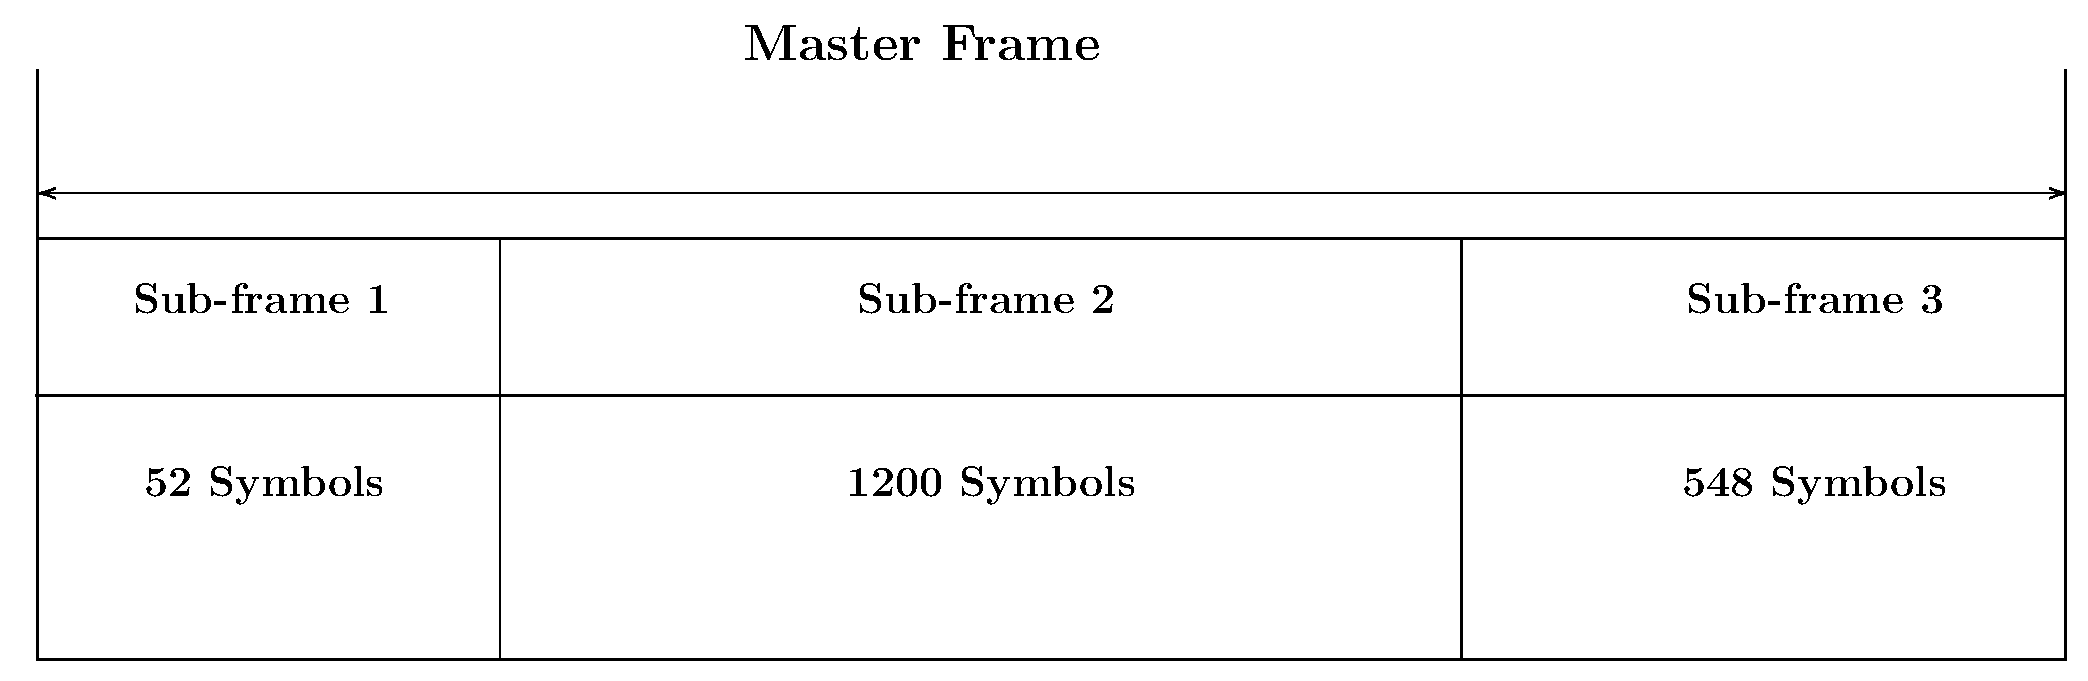
\includegraphics[width=1\columnwidth]{figs/master_frame}
\centering
\caption{Master Frame Structure}
\label{fig:master_frame}
\end{figure}

The subframe structure is as shown in Figure \ref{fig: SPS_Structure} \cite{b2}.
\begin{figure}[ht]
\centering
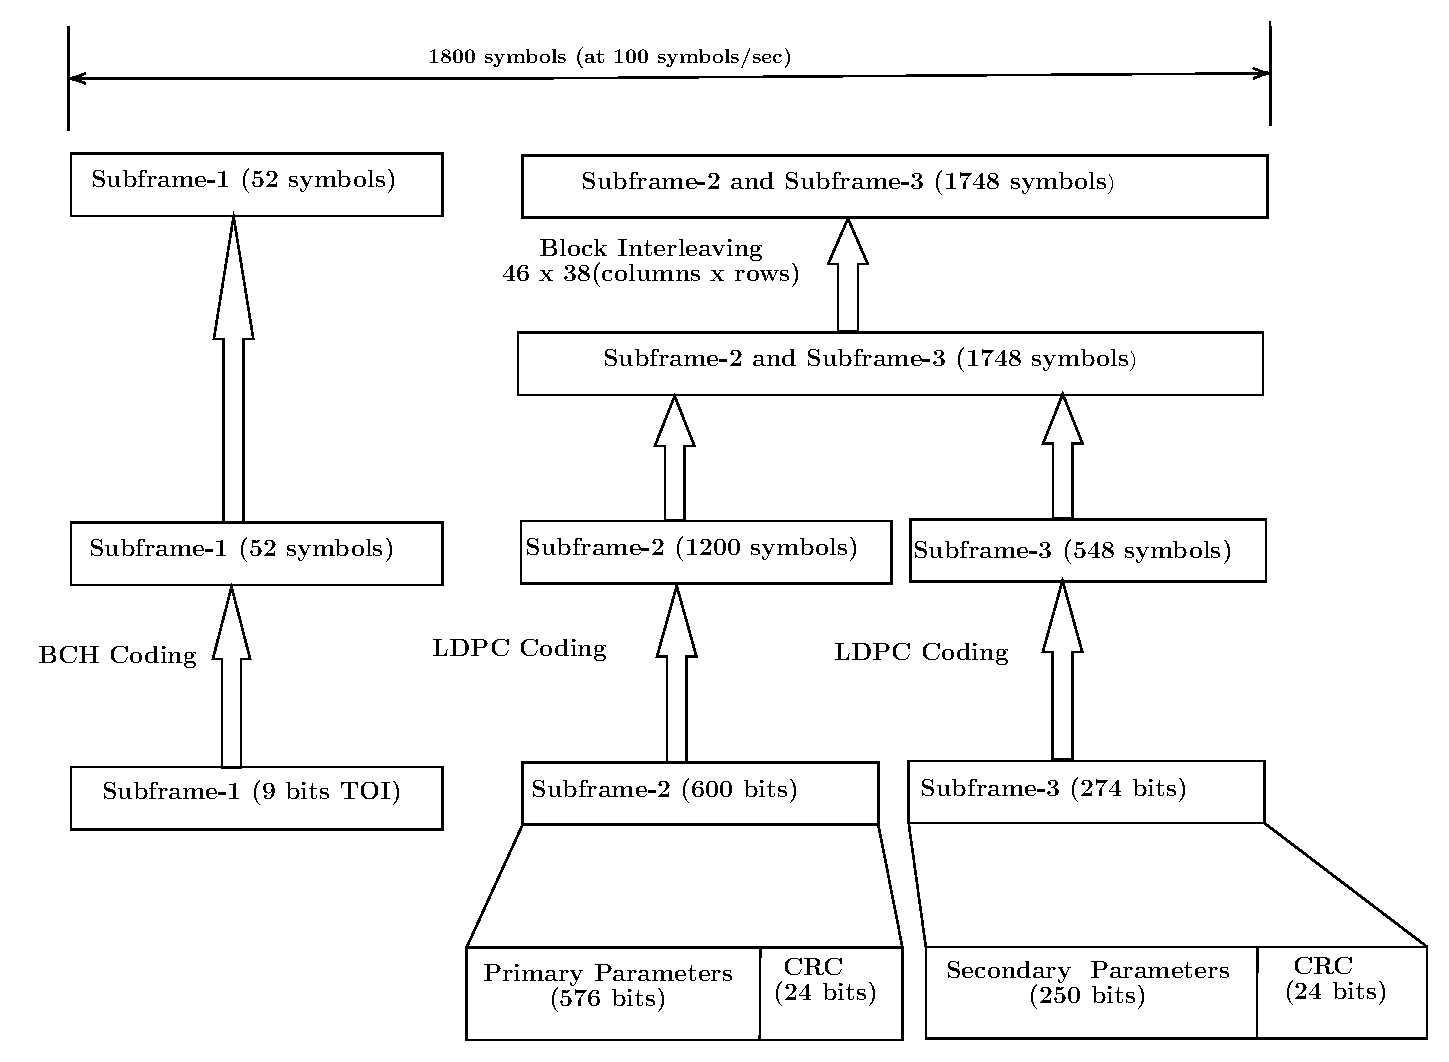
\includegraphics[width= 1\columnwidth]{figs/spsframe}
\centering
\caption{NavIC L1 SPS Subframe Structure}
\label{fig: SPS_Structure}
\end{figure}

Subframe $1$ consists of $9$ bits that are BCH encoded into 52 symbols. Subframe $2$ has 
a total of $600$ bits, comprising $576$ bits for primary navigation parameters and $24$ bits for CRC.
Subframe $3$ contains a total of $274$ bits, with $250$ bits for secondary navigation parameters and 
$24$ bits for CRC. Both subframe $2$ and subframe $3$ are separately encoded using rate $\frac{1}{2}$ 
Quasi Cyclic LDPC codes. This results in $1200$ symbols for subframe $2$ and $548$ symbols 
for subframe $3$ as shown in Figure \ref{fig: SPS_Structure}.

The CRC of data signal follows 24Q polynomial for subframe 2 and subframe 3. Any burst errors during the 
data transmission are corrected by interleaving. In matrix interleaving, input symbols are filled into a matrix 
column-wise and read at the output row-wise. Subframe 2 and subframe 3 are together interleaved using  
46 columns $\times$ 38 rows.

\subsection{PRN Codes}
Each satellite is assigned a unique PRN ranging code number, termed as PRN ID. The L1 SPS PRN 
ranging codes for both pilot and data channels associated
to a PRN ID “i” are all distinct, independent and are time-synchronized codes. 
Both these ranging codes have a period of 10230 chips which translates to 10 milliseconds
in length when operating at a chipping rate of 1.023 Mcps. 

Furthermore, the pilot channel's primary PRN code is modulated with a secondary overlay code 
with a length of 1800 and a period of 18s at a rate of 100 chips per second. The overlay codes 
for each satellite are distinct and independent. Thus, the PRN code structure for the L1 pilot 
component is that of a tiered code, that is generated by XOR-ing the primary pilot code 
with the secondary or overlay code. This is shown in Figure \ref{fig:R0_IZ4} \cite{b2}.

\begin{figure}[ht]
    \centering
    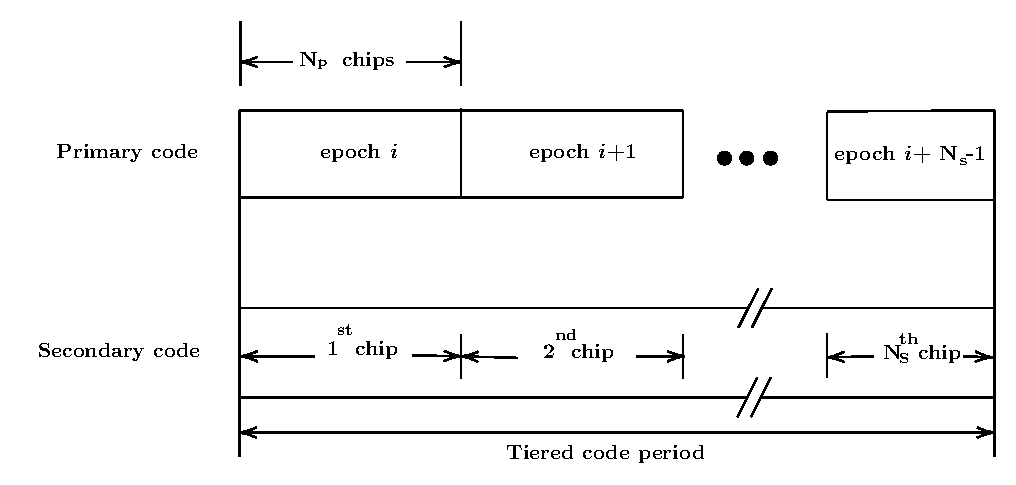
\includegraphics[width=\columnwidth]{figs/tiered_code}
    \centering
    \caption{Tiered code structure and timing relationship between primary and secondary codes}
    \label{fig:R0_IZ4}
\end{figure}
\section{Channel Modelling}
The following parameters are modelled in the satellite communication channel:
\begin{enumerate}
   \item Doppler shift
   \item Delay 
   \item Power scaling and 
   \item Thermal noise at the receiver
\end{enumerate}
\subsection{Doppler shift}
Due to relative motion between the satellites and the receiver, the transmitted signals undergo a 
frequency shift before arriving at the receiver. This shift in frequency is called Doppler shift.

The Doppler shift is introduced by muliplying the satellite signal with a complex exponential,
\begin{equation}
    x_{Shift}\sbrak{n} = x\sbrak{n}e^{-2 \pi j \brak{f_{c}+f_{Shift}} n t_{s}}
\end{equation}
where,
$x_{Shift}\sbrak{n}$ = Doppler shifted signal

$x\sbrak{n}$ = Satellite signal

$t_{s}$ = Sampling period
\subsection{Delay}
Since there is a finite distance between the satellite and the receiver, the signal at the reciever is a delayed version of the transmitted signal. This delay is given by
\begin{equation}
    D_{s} = \frac{d}{c}f_{s} 
\end{equation}
where,

$D_{s}$ = Total delay in samples

$d$ = Distance between satellite and receiver

$c$ = Speed of light

$f_{s}$ = Sampling rate

The total delay on the satellite signal is modeled in two steps. First,to introduce the static delay,
the samples are read from a queue whose size is the desired static delay length. To introduce the 
variable delay, the signal is passed throughan all-pass FIR filter with an almost constant phase 
response. Its coefficients are calculated using the delay value required.

\subsection{Power Scaling}
When a transmitting antenna transmits radio waves to a receiving antenna, the radio wave power 
received is given by,
\begin{equation}
    P_r = P_t D_t D_r \brak{\frac{1}{4 \pi \brak{f_c + f_{Shift}} D}}^2
\end{equation}
where,

$P_r$ = Received power

$P_t$ = Transmitted power

$D_t$ = Directivity of transmitting antenna 

$D_r$ = Directivity of receiving antenna 

$D$ = Total delay in seconds

To scale the received signal as per the received power calculated,
\begin{equation}
    x_{Scaled}\sbrak{n} = \frac{\sqrt{P_r}}{\operatorname{rms}\brak{x\sbrak{n}}}x\sbrak{n}
\end{equation}   

\subsection{Thermal noise}
The thermal noise power at the receiver is given by,
\begin{equation}
    N_r = k T B
\end{equation}
where,

$N_r$ = Noise power in watts

$k$ = Boltzmann's constant

$T$ = Temperature in Kelvin

$B$ = Bandwidth in Hz

AWGN (Additive White Guassian Noise) samples with zero mean and variance $N_r$ are generated and added to the satellite signal to model thermal noise at receiver.

\section{Software Implementation of Receiver}
The block diagram of the receiver is as shown in Figure \ref{fig:demod_flow}.
\begin{normalsize}
	\begin{figure}[ht]
		\centering
		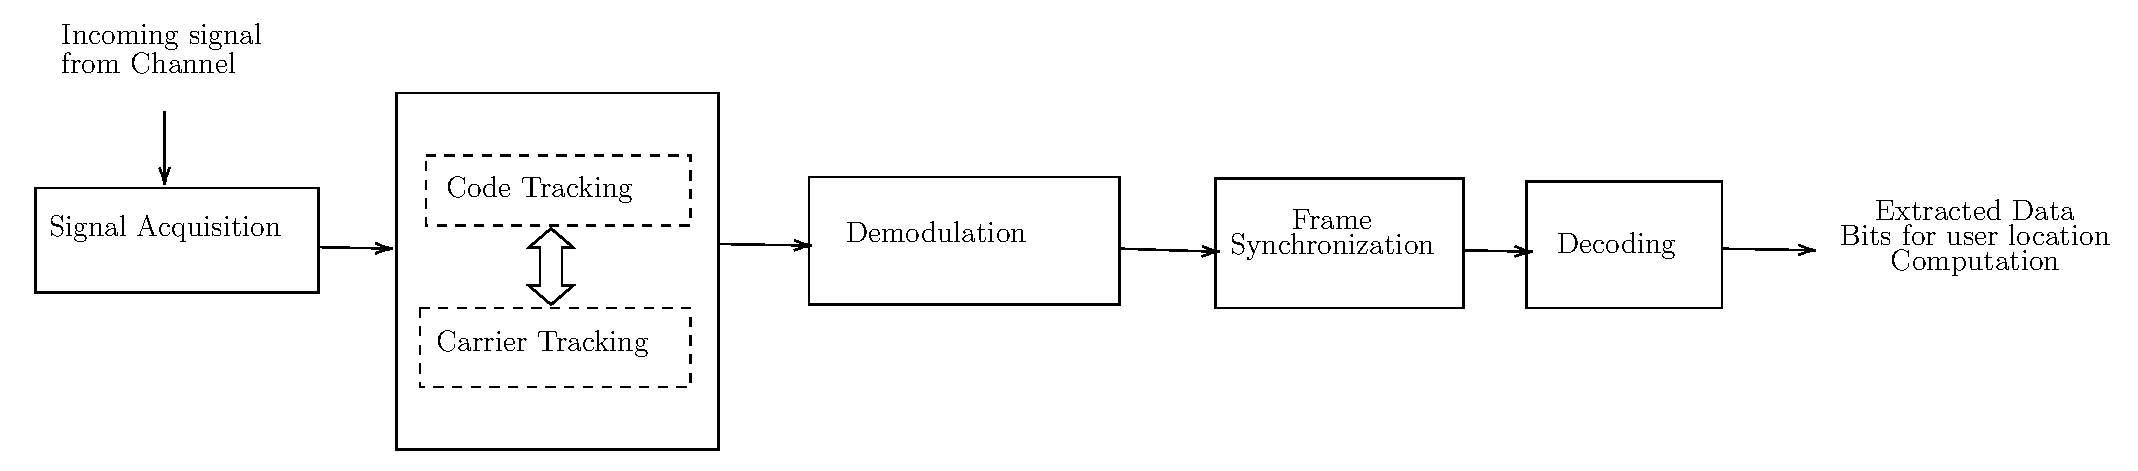
\includegraphics[width=1\columnwidth]{figs/receiver_block}
		\centering
		\caption{The Block Level Architecture for Receiver}
		\label{fig:demod_flow}
	\end{figure}
\end{normalsize}

The signal processing chain at the receiver is divided into five steps:
\begin{enumerate}
	\item Acquisition
	\item Tracking
	\begin{enumerate}
		\item Carrier Tracking
		\item Code Tracking
	\end{enumerate}
	\item Demodulation
	\item Frame synchronisation
	\item Channel decoding
\end{enumerate}

\subsection{Acquistion}

A generic NavIC L1 SPS signal is defined by its complex baseband equivalent, 
$S_T(t)$, the digital signal at the input of an Acquisition block can be written as:
\begin{multline}
	x_{IN}[k]=A(t)\hat s_T (t-\tau(t))e^{j(2 \pi f_D(t)t+\Phi(t))}\bigg|_{t=kT_s} \\ 
    +n(t)\bigg|_{t=kT_s}
\end{multline}

\noindent where $f_D$ is Doopler shift frequency, $\tau$ is PRN Code delay,$\Phi$ is Phase shift
and $n(t)$ is AWGN noise. 

The role of the acqusition block is to examine the presence/absence of signals coming from a 
given satellite. In the case of signal being present, it should provide coarse estimations of the 
Code delay ($\tau$) and the Carrier Doppler shift ($f_D$), yet accurate enough to initialize the carrier and code 
tracking loops.

\subsubsection{Implementation of PCPS Acquisition}
The Parallel Code Phase Search (PCPS) algorithm \cite{b1},\cite{b3} is used in Acquisition block 
and is shown in Figure \ref{fig:pcps_flow}. in the 2-dimnesional search, the frequency bin having 
maximum input signal power is determined as coarse doppler frequency ($f_D$). 
The index at which the peak power is present in that frequency bin is termed as coarse Code delay 
($\tau$). These values are 
passed to the Tracking module. If the Input signal power is less than a threshold, then the 
satellite is 
considered to be non-visible. Under low SNR conditions, samples from 2-3 successive coherent 
integration periods can be added to have a better acquisition sensitivty.

\begin{normalsize}
\begin{figure}[ht]
	\centering
	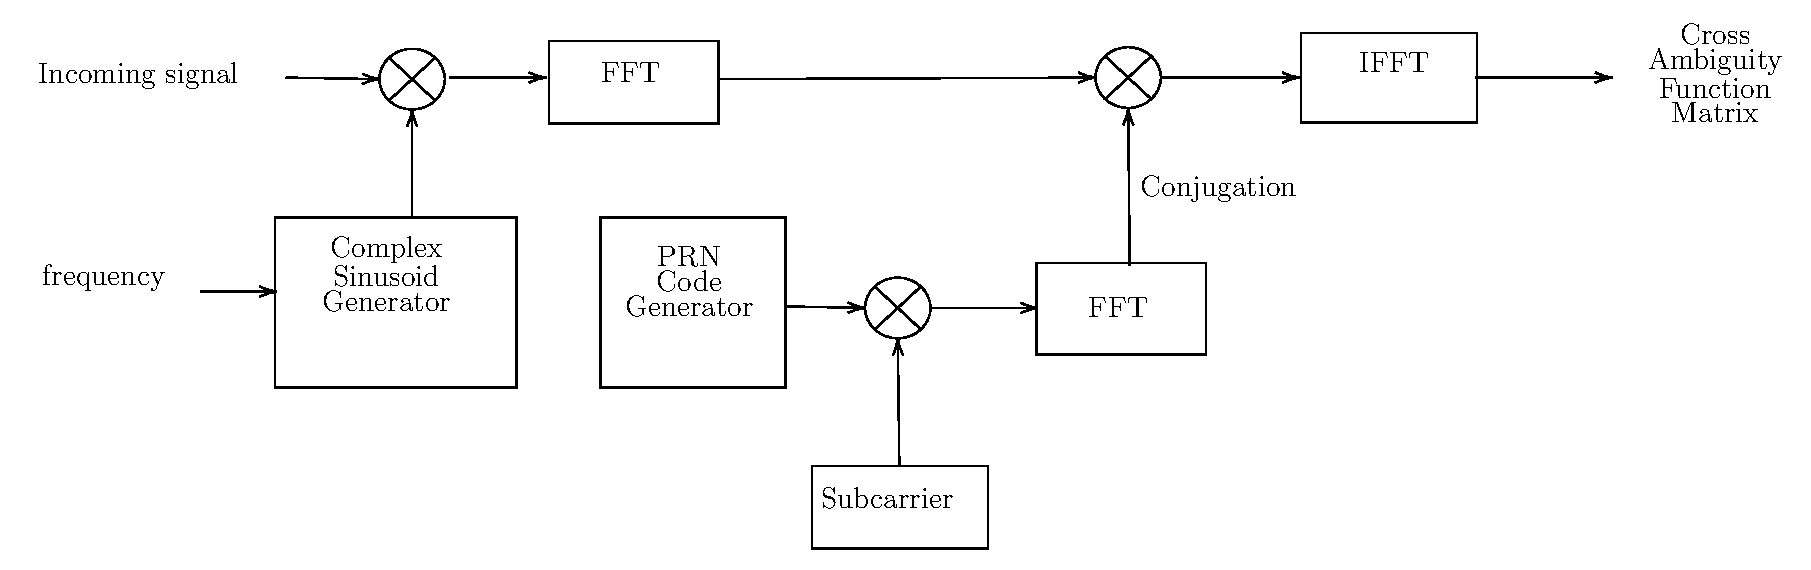
\includegraphics[width=1\columnwidth]{figs/pcps}
	\centering
	\caption{PCPS algorithm flow}
	\label{fig:pcps_flow}
\end{figure}
\end{normalsize}

\subsection{Tracking}
The role of tracking block \cite{b5} is to refine coarse estimations and follow signal synchronization parameters: code phase, Doppler shift 
and carrier phase and extract the baseband signal. It performs the following 3 functions to decipher 
the baseband signal from the incoming signal as shown in figure \ref{fig:tracking}. The tracking algorithm 
specified in \cite{b1} is used in this work.
\begin{enumerate}
	\item Carrier and code wipeoff 
	\item Pre-detection integration
	\item Baseband signal processing
\end{enumerate}

\begin{normalsize}
\begin{figure}[ht]
\centering
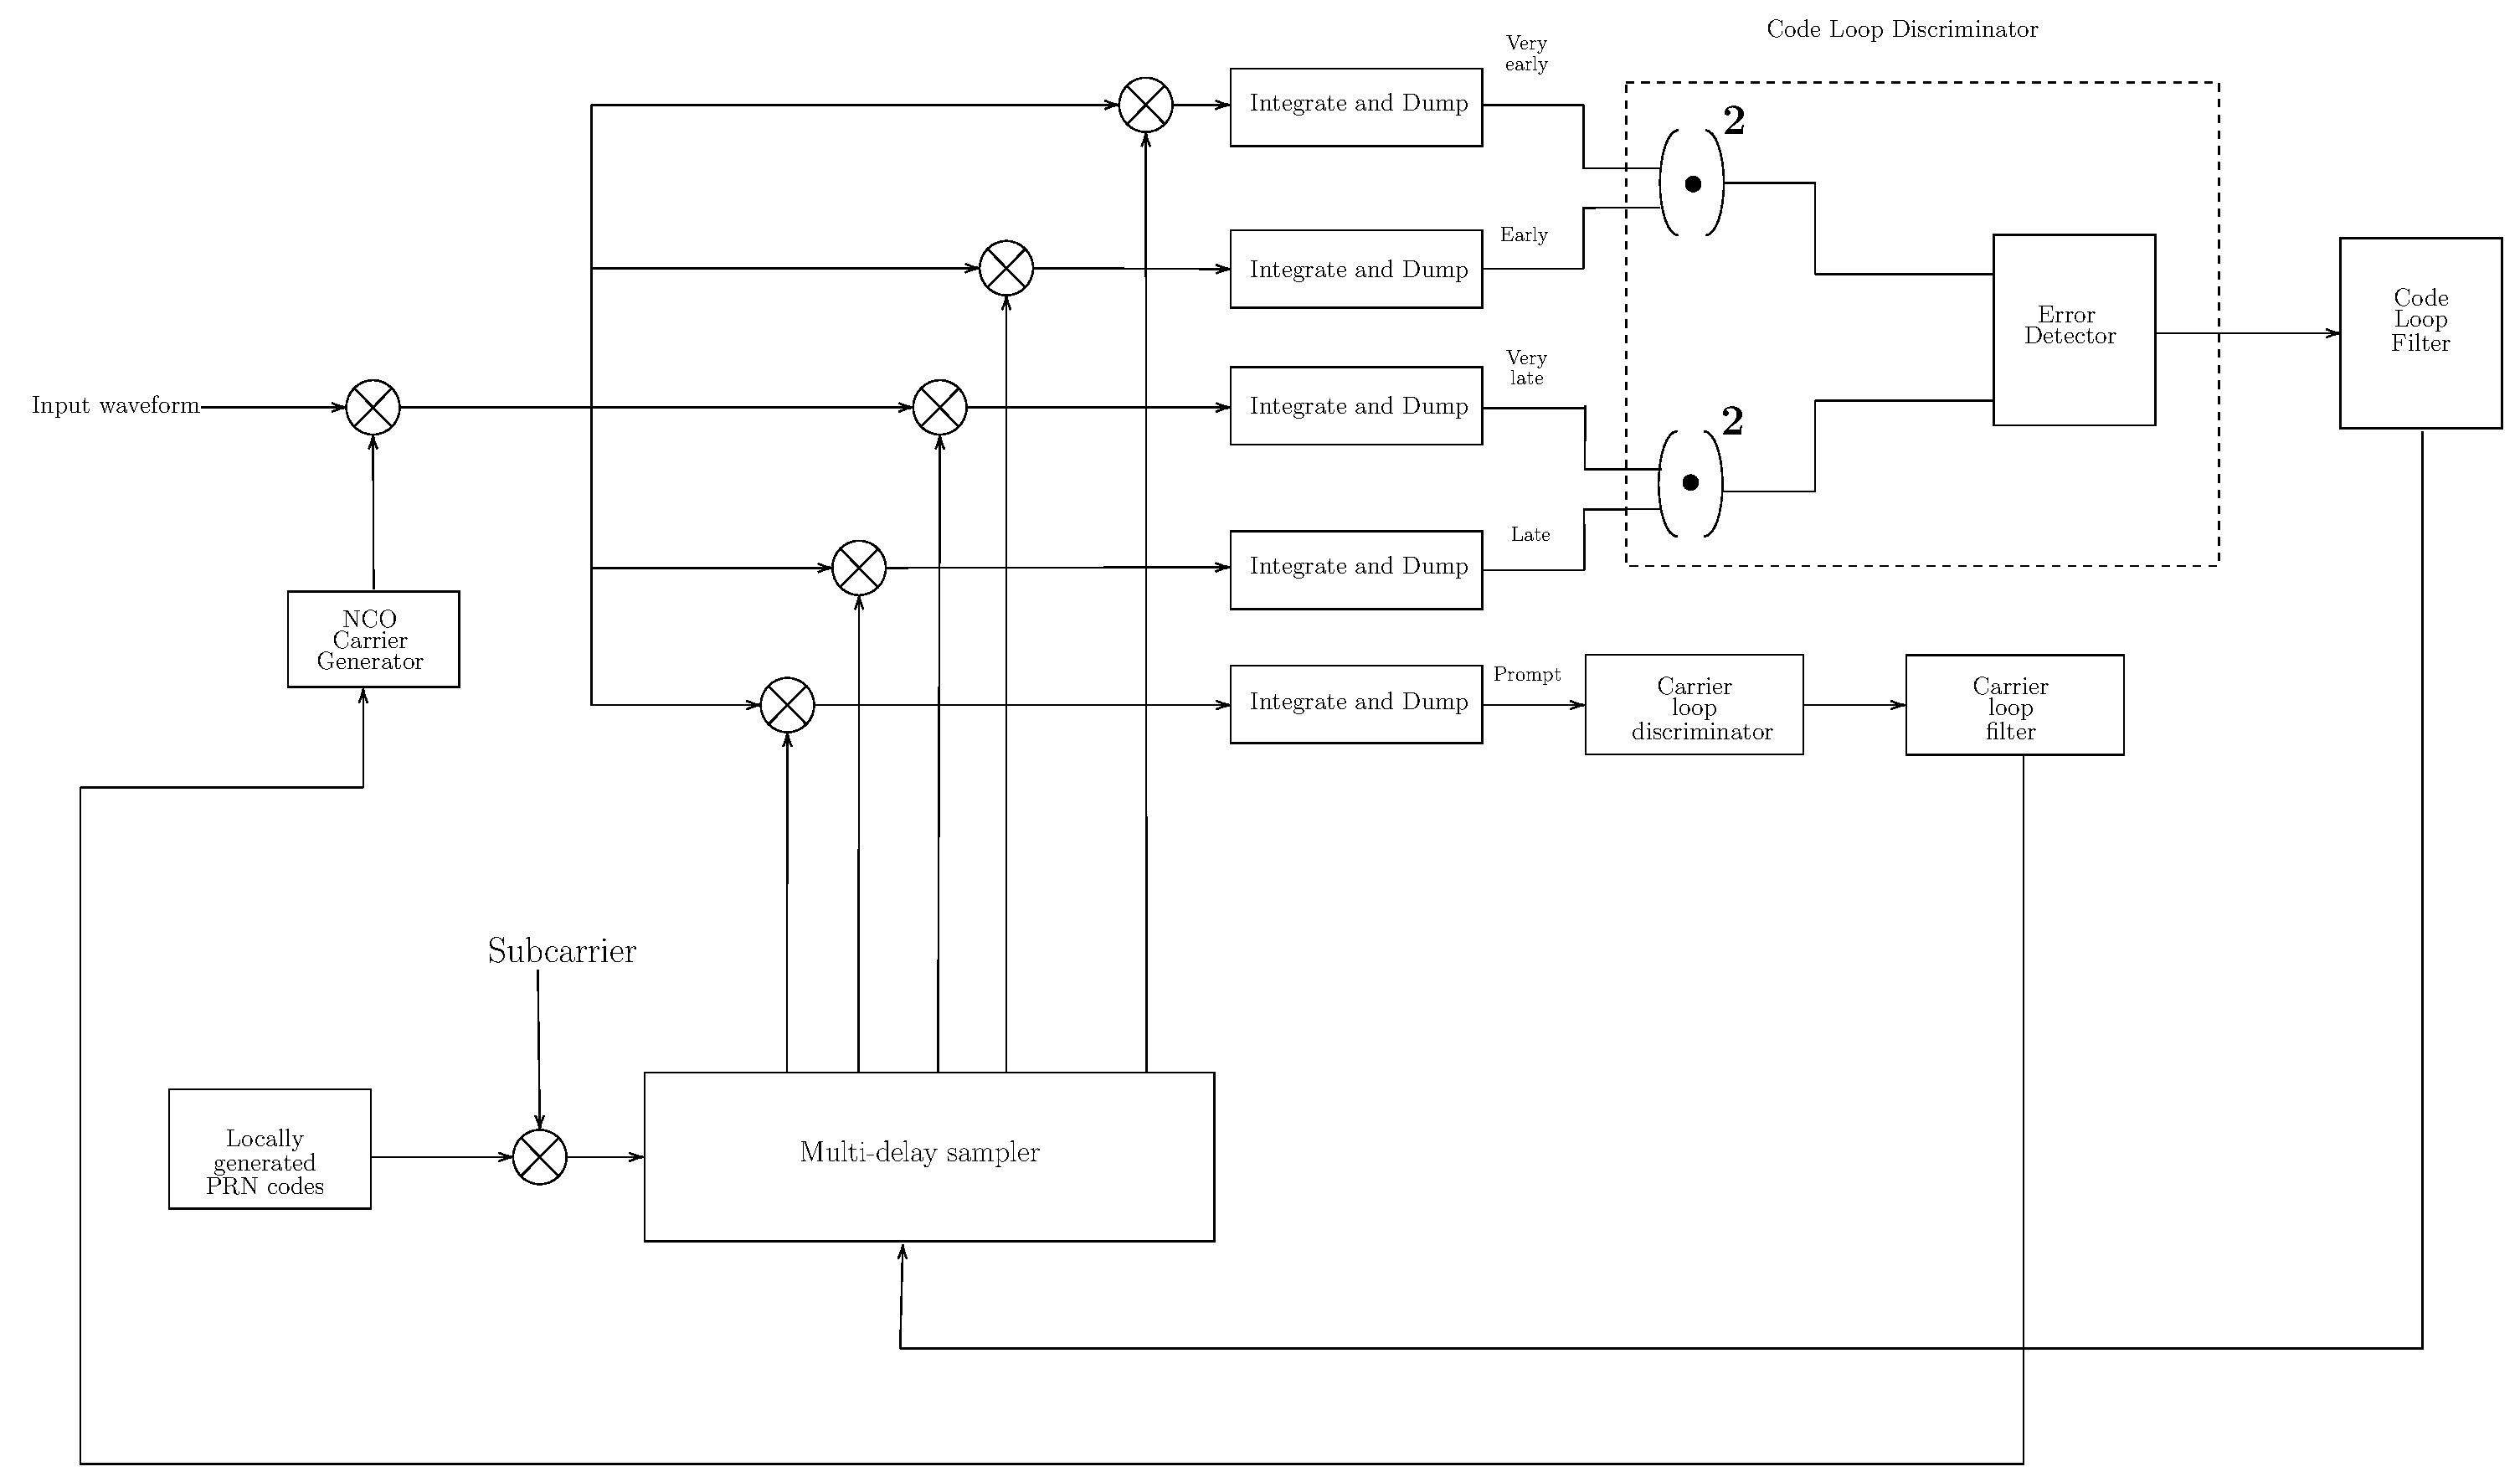
\includegraphics[width=1\columnwidth]{figs/tracking}
\centering
\caption{Tracking block diagram}
\label{fig:tracking}
\end{figure}
\end{normalsize}
\subsubsection{Carrier and code wipeoff}
\textbf{Carrier wipeoff: }Referring to the Figure \ref{fig:tracking}, first, the incoming signal is 
stripped off the carrier (plus carrier Doppler) by a local replica carrier (plus carrier Doppler) 
signals. The replica carrier (including carrier Doppler) signals are synthesized by the carrier 
numerically controlled oscillator (NCO). In closed loop operation, the carrier NCO is controlled 
by the carrier tracking loop in the receiver processor.
\\
\textbf{Code wipeoff: }ACF of BOC signal contains 2 locals maximas, apart from having a global maxima at $0^{th}$ chip delay.
To detect these maximas, the received signal is  correlated with Very Early(VE), Early(E), 
Prompt(P), Late(L) and Very Late(VL) local replica codes (plus code Doppler) synthesized by a 
multi-delay sampler. In the closed loop operation, the code NCO is controlled by the code tracking 
loop in the receiver processor. E and L are typically separated in phase by 0.3 chips. VE and VL are
separated by 1.2 chips. The prompt replica code phase is aligned with the 
incoming satellite code phase producing maximum correlation if it is tracking the incoming satellite code 
phase.  Any misalignment in the replica code phase with respect to the incoming code phase produces 
a difference in the vector magnitudes of the VE,E,L and VL correlated outputs so that the amount 
and direction of the phase change can be detected and corrected by the code tracking loop.
\subsubsection{Pre-detection and integration}
Extensive digital predetection integration and dump processes occur after the carrier and code 
wiping off processes. Figure \ref{fig:tracking} shows five complex correlators required to produce 
five components, which are integrated and dumped to produce VE,E,P,L,VL vesions of the signal.
\subsubsection{Baseband signal processing}
This entails Carrier tracking and Code tracking using Phase locked loop (PLL), Frequency locked loop
(FLL) and Delay locked loop (DLL). \\

\noindent\textbf{Phase locked loop(PLL)}\\
The carrier loop discriminator defines the type of tracking loop as a PLL, a Costas PLL 
(which is a PLL-type discriminator that tolerates the presence of data modulation on the baseband 
signal), or a frequency lock loop (FLL). Carrier tracking loop tracks the frequency and phase of 
the received signal by detecting the phase error between replicated signal and incoming signal. 
This error is fed through loop filter to Carrier NCO so as to adjust its frequency and phase to 
synchronize with incoming signal in both frequency and phase. For very low phase error detected, 
navigation data is accurately extracted. 
\begin{align}
  %\text{Phase error} =ATAN2(I_P,Q_P) = \tan^{-1}\brak{\frac{I_P}{Q_P}}
  \text{Phase error}_{pilot} &=ATAN2(I_P,Q_P) = \tan^{-1}\brak{\frac{I_P}{Q_P}}
\end{align}
\\
\\
\noindent\textbf{Frequency locked loop}\\
PLLs replicate the exact phase and frequency of the incoming signal to perform the 
carrier wipeoff function. FLLs perform the carrier wipeoff process by replicating the approximate 
frequency, and they typically permit the phase to rotate with respect to the incoming carrier signal.
The algorithm used in FLL discriminator is $\frac{\text{ATAN2}{\brak{cross,dot}}}{t_2-t_1}$. 
The frequency error is given by 
\begin{align}
	\text{Frequency error} = \frac{\phi_2-\phi_1}{t_2-t_1}
\end{align}

\noindent The phase change $\phi_2 - \phi_1$ between two adjacent samples of $I_{P}$ and $Q_{P}$ 
at times $t_2$ and $t_1$ is computed. This phase change in a fixed interval of time is proportinal 
to frequenct error in the carrier tracking loop. The error is fed to carrier NCO through a loop filter 
to adjust the frequency to lock to the right frequency.


\noindent\textbf{Delay locked loop:}
Post the carrier signal synchronization, received code samples are synchronized by aligning 
with locally replicated code samples by shifting right or left. To determine the direction of shift, 
the I and Q outputs are multiplied with prompt code (PRN code which is phase aligned), 
E and VE code (prompt PRN code shifted by some samples to the left) and L,VL code (prompt PRN code 
shifted by some samples to the right) resulting in corresponding I and Q channel respectively. 
Following algorithm is used to lock the code phase.

\begin{align}
	E_K&=\sqrt[]{VE^2+E^2}\\
	L_K&=\sqrt[]{VL^2+L^2}
\end{align}

\begin{align}
	\text{DLL Discriminator} (\epsilon)&=\frac{1}{2}\frac{E_K-L_K}{E_K+L_K}
\end{align}

\noindent If the replica code is aligned, then the E $\&$ L and VE $\&$ VL envelopes are equal in 
amplitude and no error is generated by the discriminator. If the replica code is misaligned, then 
code phase error is sensed by code discriminator. This error is filtered and 
then applied to the code loop NCO, where the output code shift is increased or decreased as 
necessary to correct the replica code generator phase with respect to the incoming  signal code 
phase.

\noindent When tracking loop is in locked state, $I_P$ component of Data channel will carry Data 
sysmbols and $Q_P$ of Pilot channel will carry pilot overlay codes.

\subsection{Demodulation}
After the aquisition and tracking have been performed, the received data is mapped back using BPSK 
demodulation, mapping $-1$ to binary $1$ and $+1$ to binary $0$. Data symbols and Pilot 
overlay codes are obtained after demodulation process.

\subsection{Frame synchronisation}
The start of master frame for a given satellite is determined using correlation of 
recevied pliot overlay bits with locally generated pilot's overlay bits. The index at which the 
maximum correlation output is present is considered as the start of master frame. The same
index is used to decode the data symbols.

\subsection{Decoding}
Demodulated data is first separated into subframes using the frame index. Subframe 1 is decoded 
using Maximum-likelihood method (BCH decoding). Subframes 2 and 3 are deinterleaved and decoded 
using belief propagation (LDPC decoding) \cite{b6}. CRC is calculated to verify if there are any errors. 
\subsubsection{Process}
The high-level diagram of the channel decoding process in NavIC L1 is shown in Figure 
\ref{fig:decoding_r}.
\begin{normalsize}
\begin{figure}[ht]
\centering
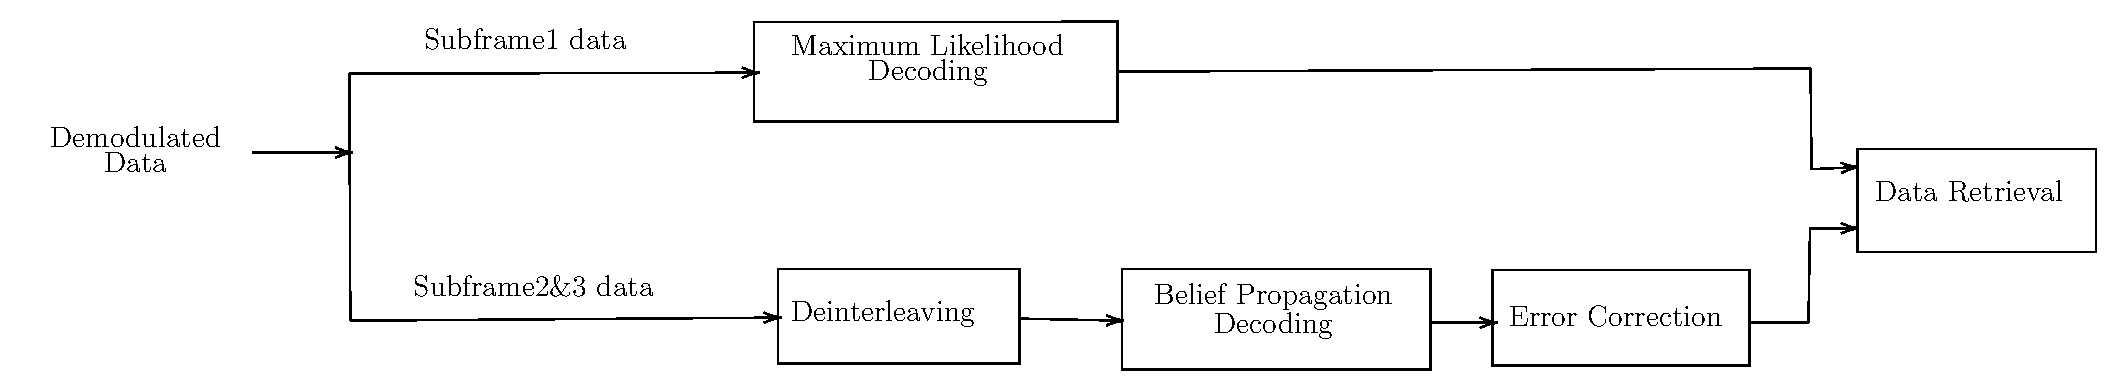
\includegraphics[width=1\columnwidth]{figs/decoding_r}
\centering
\caption{The Block Level Architecture for Channel decoding}
\label{fig:decoding_r}
\end{figure}
\end{normalsize}

\section {Simulation results}
\subsection{Transmitter}
The simulation of transmitter starts with generating Pilot PRN codes(primary and secondary) $\&$ 
Data PRN codes for 4 satellites and upsampling them with sampling frequency $F_s$ of $4$MHz.  
Navigation bits for Master frames are randomly generated, CRC is padded and necessary encoding and 
interleaving are carried out to generate symbols for $3$ subframes. $36$ seconds of sample data 
is generated for each of the satellites($36\times4$M samples). Baseband signal for each of the 
satellites is generated as per the modulation scheme. For each of these signals, doppler shift 
(between $-5000$Hz to $5000$Hz), code delay($0-10230$) and power scaling are applied. 
The composite signal is generated by adding all these 4 signals. AWGN noise (-20dB to 0dB) is added
to this signal resulting in an SPS L1 signal. This simulated sigaml is transmitted (without carrier)
through the channel.
\subsection{Receiver}
The symbol period of 10ms is considerd as Integration period at the receiver end. In the receiver 
module, Acquisition block reads 10ms of received samples (N= 40,000) and finds out visible 
satellites and coarse Doppler shift ($F_d$) $\&$ coarse Code delay($\tau$) using PCPS algorithm. 
Frequency search band of -5000Hz to 5000Hz with a step size of 80Hz is used for this purpose.  
PCPS output shown in Figure \ref{fig:acq_output} for a satellite, depicts received signal for 
various doppler frequencies and code delay. 

\begin{figure}[ht]
	\centering
	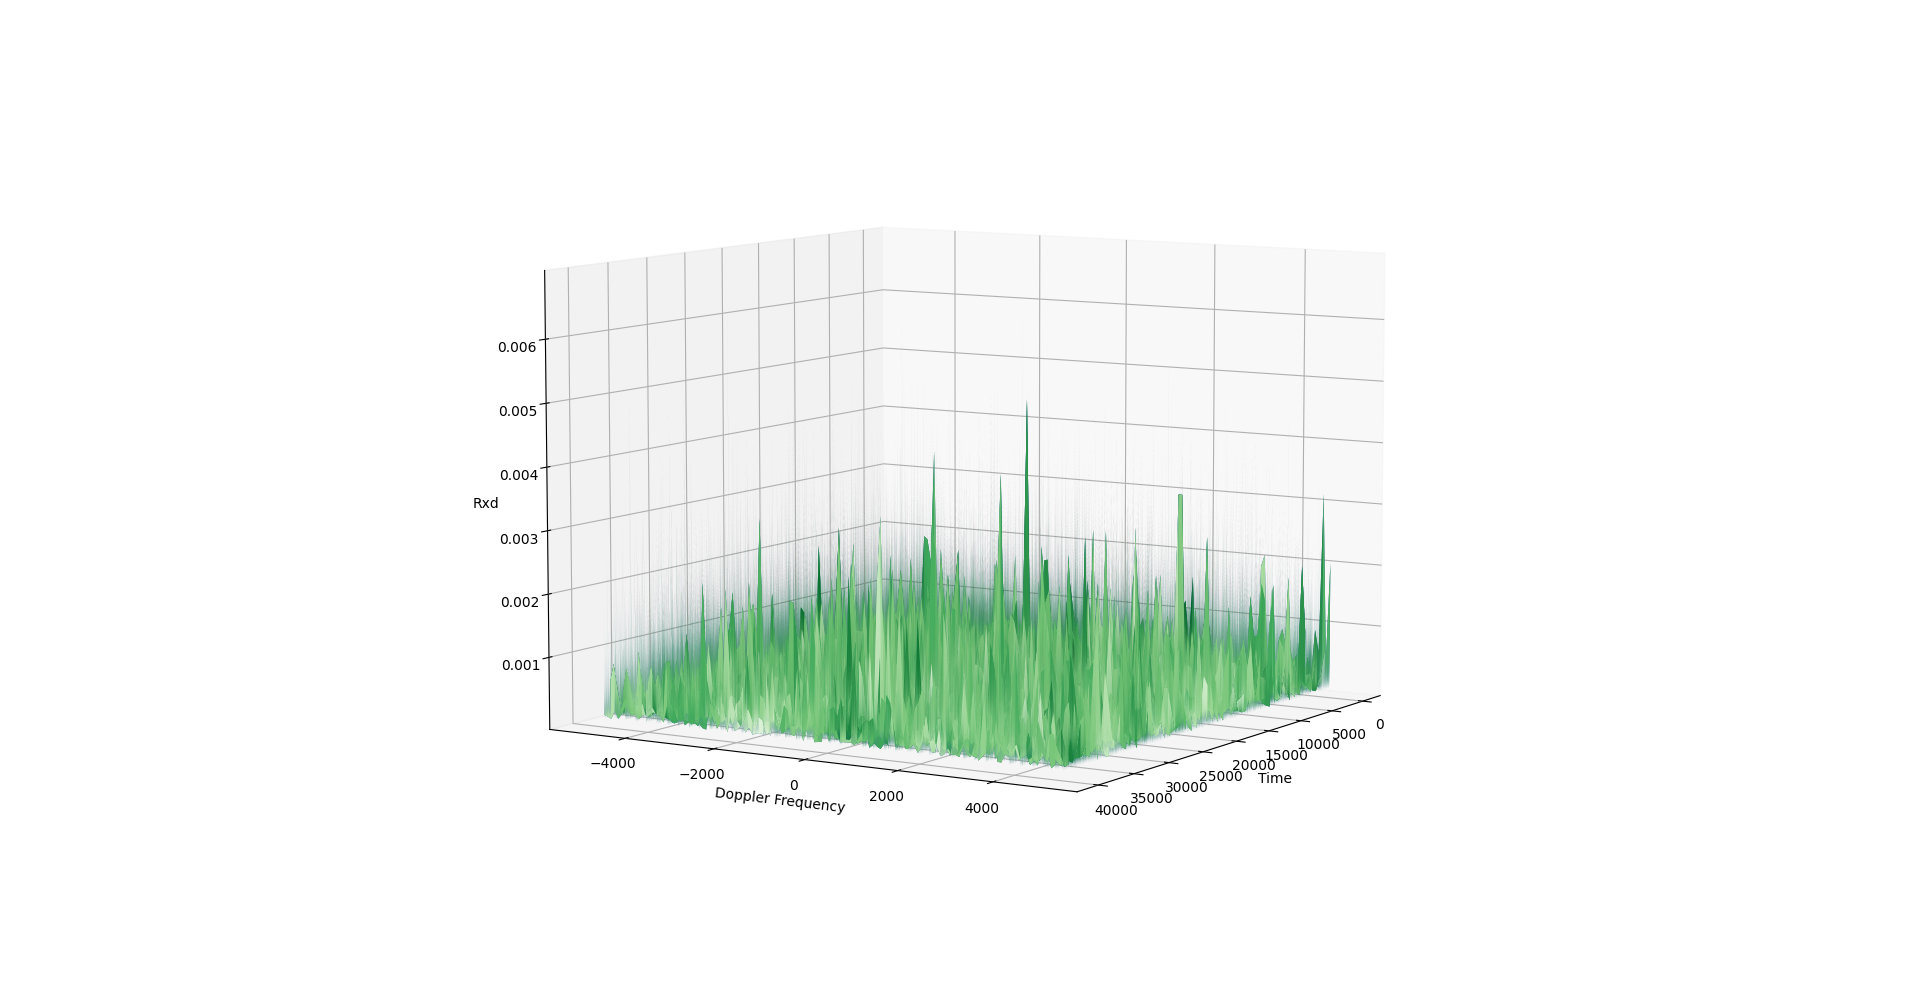
\includegraphics[width=1\columnwidth]{figs/acq_output.png}
	\centering
	\caption{Received signal Power vs Frequnecy \& Code delay}
	\label{fig:acq_output}
\end{figure}

Acquisition results for 4 satellites are as shown below
\begin{lstlisting}[mathescape=true]
	Acquisition results for $\textbf{PRN ID 2}$
	Peak to noise ratio= 16.82
 	Status:True Doppler:520 Delay/Code-Phase:301
	Acquisition results for $\textbf{PRN ID 3}$
	Peak to noise ratio= 10.93
 	Status:True Doppler:1320 Delay/Code-Phase:588
	Acquisition results for $\textbf{PRN ID 4}$
	Peak to noise ratio= 14.46
 	Status:True Doppler:3800 Delay/Code-Phase:426
	Acquisition results for $\textbf{PRN ID 6}$
	Peak to noise ratio= 17.74
 	Status:True Doppler:4920 Delay/Code-Phase:313
\end{lstlisting}

The tracking loop runs for 3600 times ($36\times100$ symbols/sec) to process received samples for 
each satellite. Tracking loop uses the following parameters:
\begin{enumerate}
	\item Buffer size for power estimation = 10
	\item  $CN0_{min}$ = 25
	\item Phase lock detector threshold = 0.85
	\item Lock fail counter threshold = 25 
	\item Lock counter threshold = 20
	\item PLL Noise Bandwidth = 18 Hz
	\item FLL Noise Bandwidth = 2 Hz
	\item DLL Noise Bandwidth = 2 Hz
	\item SNR = -10db
\end{enumerate}
Figure \ref{fig:tracking_output} shows tracking output for a satellite detailing Frequency, Phase and Code delay error and NCO output values.
\begin{figure}[ht]
	\centering
	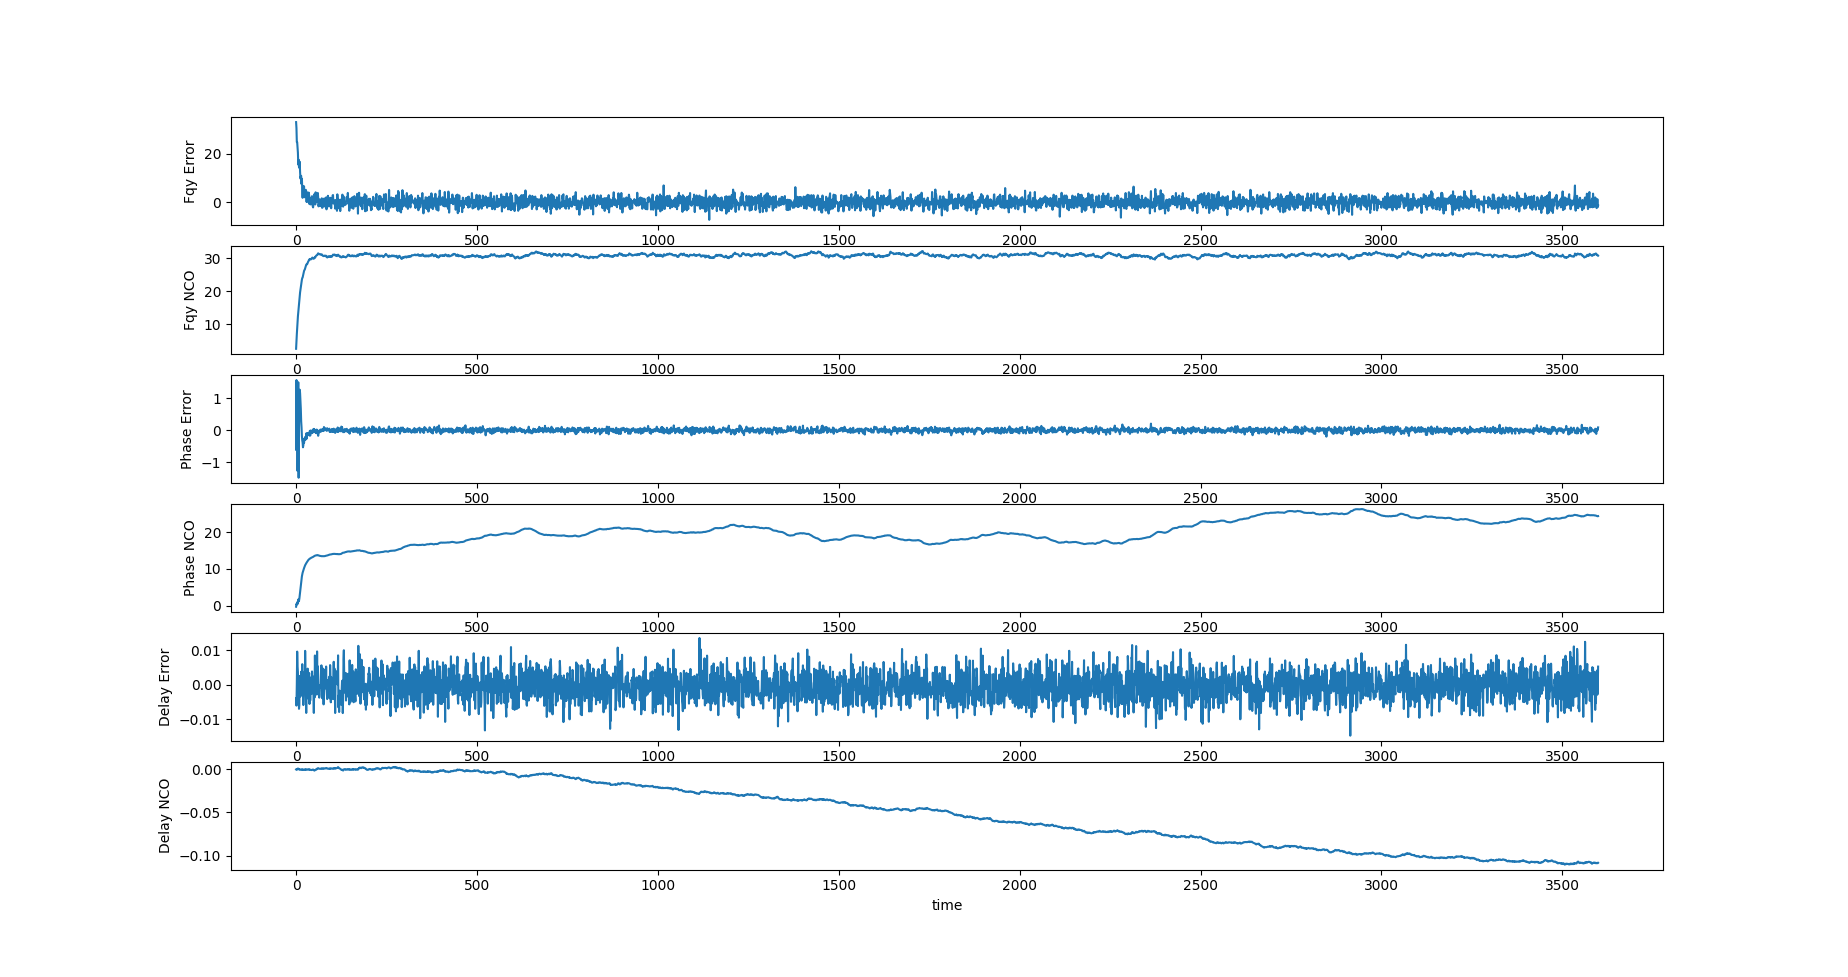
\includegraphics[width=1\columnwidth]{figs/tracking_output.png}
	\centering
	\caption{Tracking output}
	\label{fig:tracking_output}
\end{figure}

Figure \ref{fig:navbits_output} shows, for a satellite, NAV bits transmitted and received for Subframes 1,2 and 3. 
For subframe 1, all 9 bits are shown while for subframes 2 and 3, first 24 bits are shown.

\begin{figure}[ht]
	\centering
	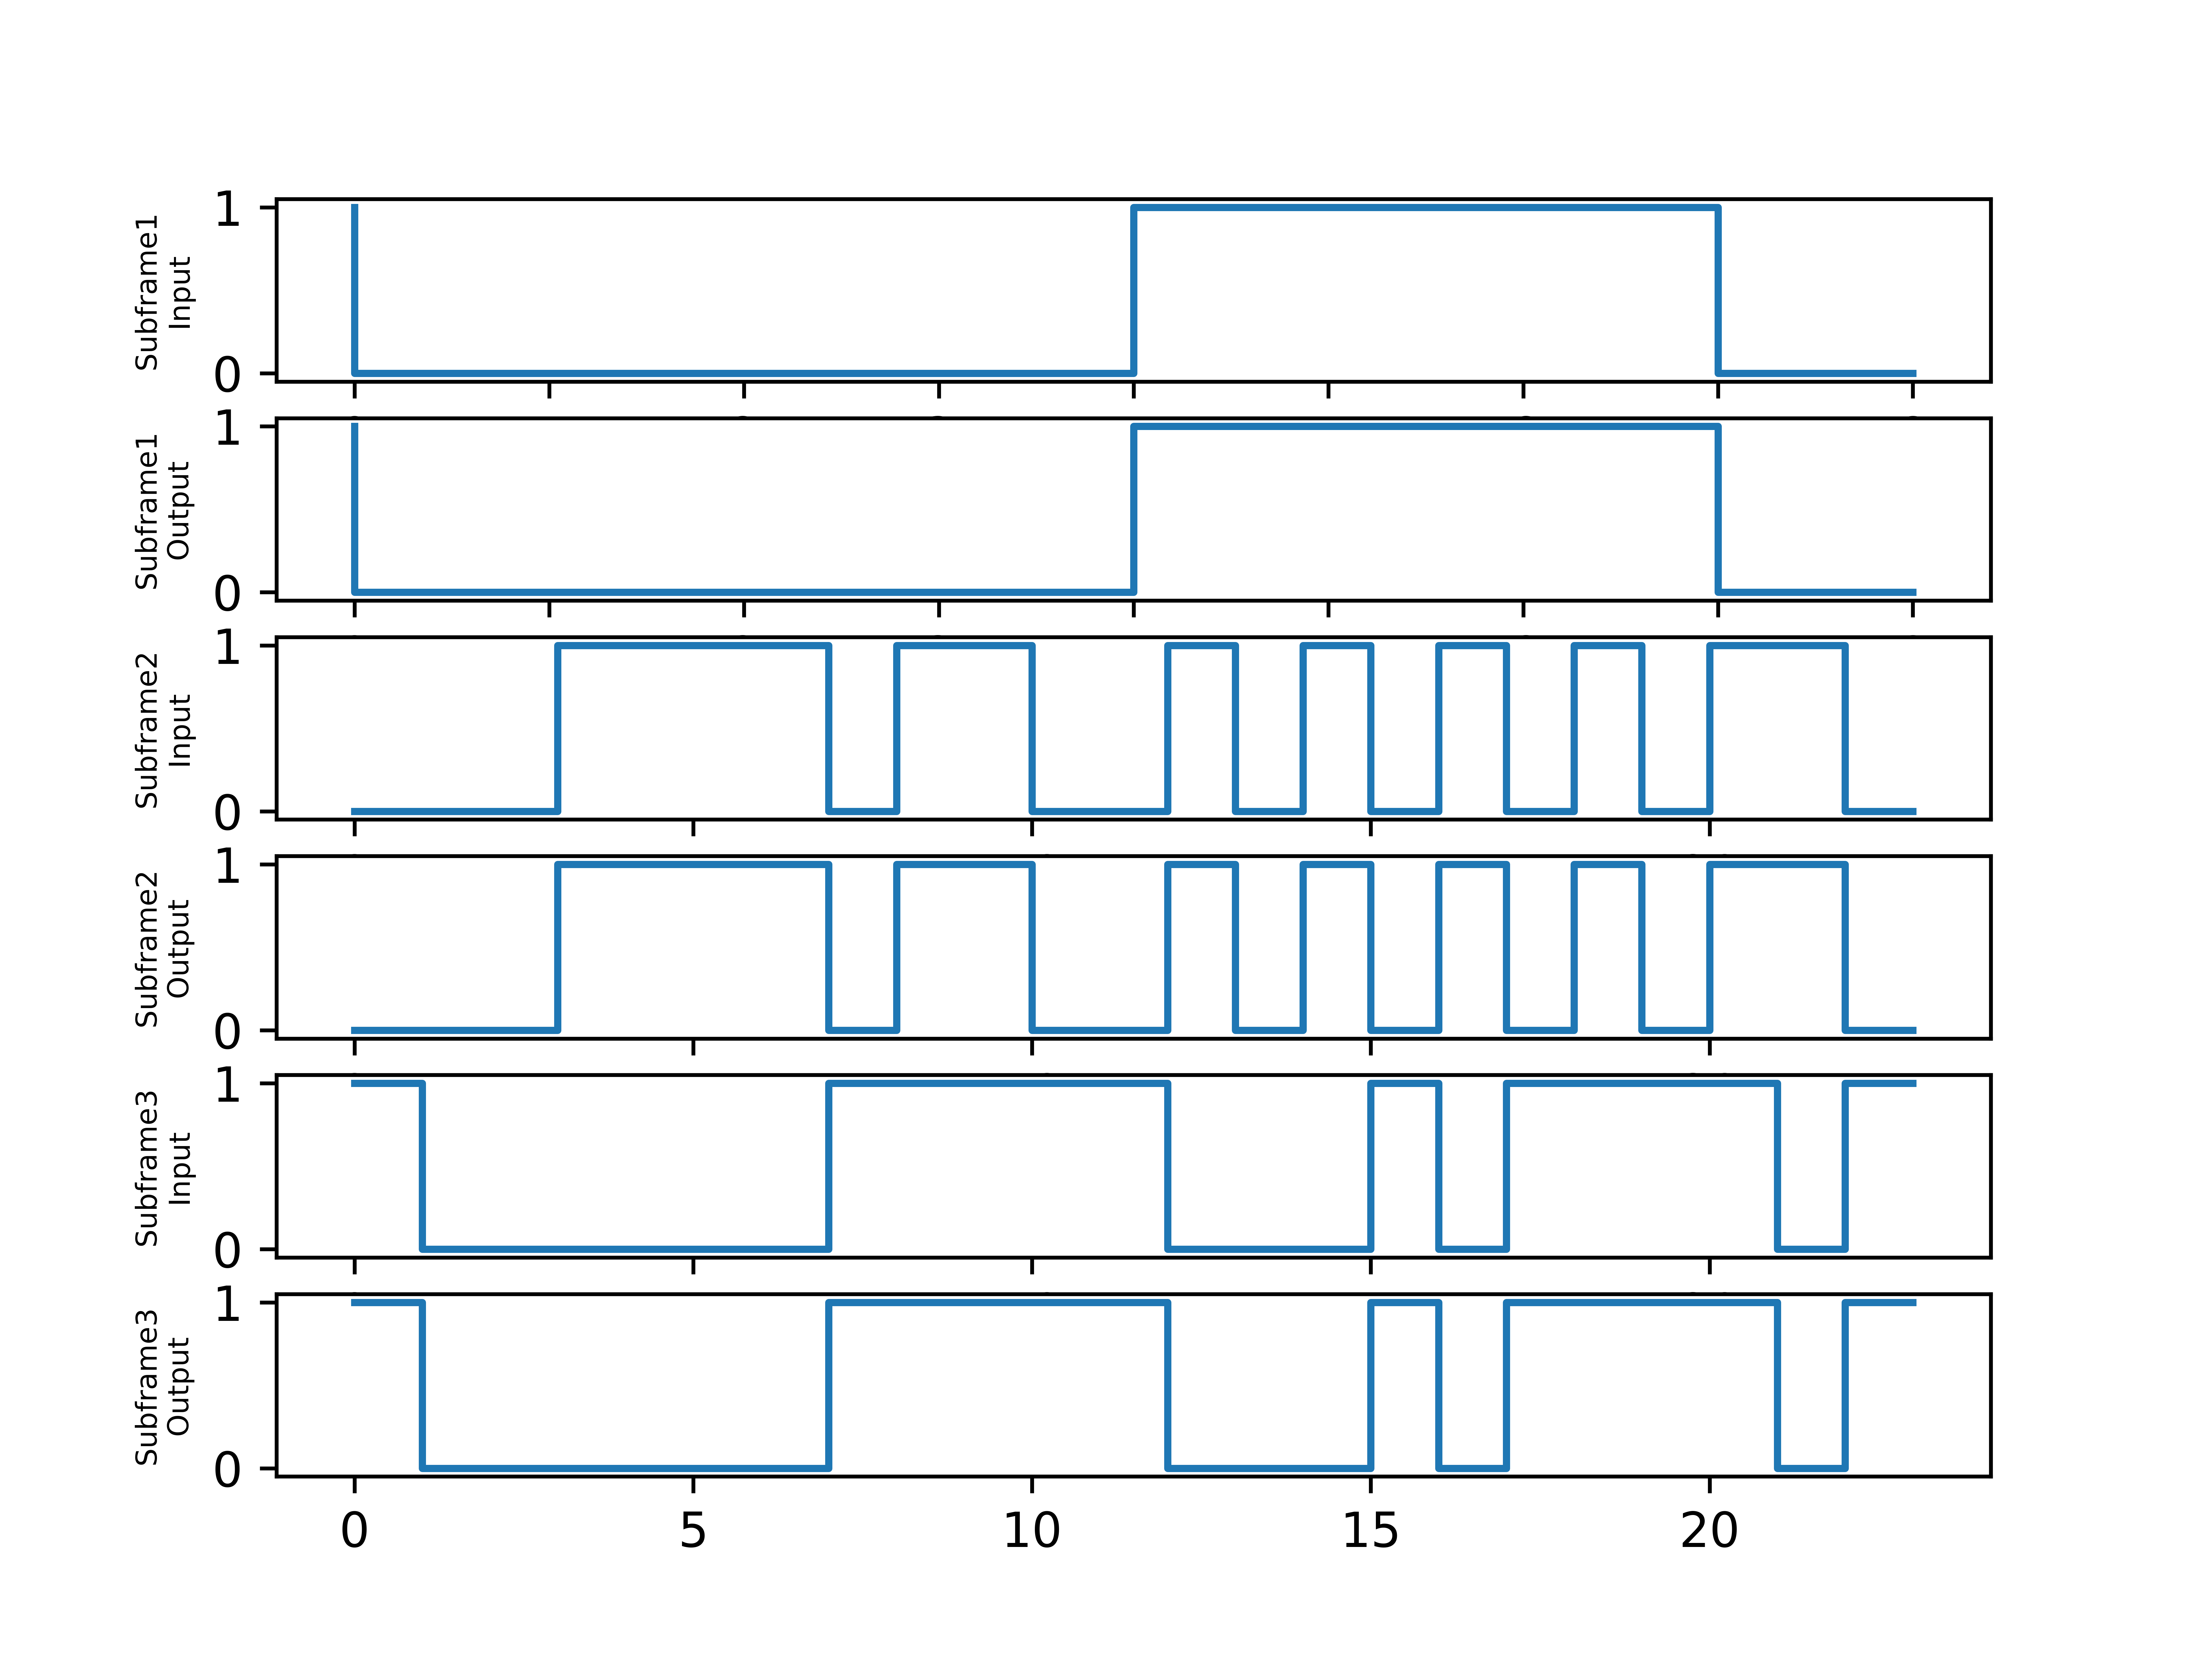
\includegraphics[width=0.75\columnwidth]{figs/mynavbits.png}
	\centering
	\caption{NAV bits transmitted and received}
	\label{fig:navbits_output}
\end{figure}

\section {Future work}
The current work has focused on proper reception of NavIC L1 SPS baseband signal. In future work, 
the receiver should be fed with I and Q samples from a NavIC L1 simulator (ISRO had built a 
simulator) to calculate user location. Subsequetly, when a minimum of 4 NavIC satellites with L1 
band are available in constellation, the receiver has to be tested with real time data received 
from satellite.
\section {Conclusions}
In this paper, we presented open source implemnetation in Python of generating SPS NavIC L1 baseband 
signal, transmitting it through a modelled channel and processing the received data for accurate reception.
Various singal processing blocks like Acquisition, trackng and decoding  etc are discussed in detail. The open source
code and documentation is available at https://github.com/satheeshsimha/navic-1/tree/main/L1.

\begin{thebibliography}{00}
\bibitem{b1} Carles Fernández-Prades,Javier Arribas,Luis Esteve,David Pubill,Pau Closas, "An open source Galileo E1 software receiver", Published in: 2012 6th ESA Workshop on Satellite Navigation Technologies (Navitec 2012) $\&$ European Workshop on GNSS Signals and Signal Processing held from 05-07 December 2012.
\bibitem{b2} NavIC Signal In Space ICD for SPS in L1 frequency, V1.0, October 2022,https://www.isro.gov.in/media\_isro/pdf/Publications/Vispdf/Pdf2017/\\1a\_messgingicd\_receiver\_incois\_approved\_ver\_1.2.pdf
\bibitem{b3} GNSS SDR documention on Acquisition, https://gnss-sdr.org/docs/sp-blocks/acquisition/
\bibitem{b4} GNSS SDR documentation on Tracking, https://gnss-sdr.org/docs/sp-blocks/tracking/
\bibitem{b5} Elliott D. Kaplan and Christopher J. Hegarty,  "Understanding {GPS} {P}rinciples and {A}pplications", $3^{rd}$ edition
\bibitem{b6} Lingxia Zhou, Meixiang Zhang, Satya Chan 2 and Sooyoung Kim, "Review and Evaluation of Belief Propagation Decoders for Polar Codes", Symmetry2022, 14, 2633. https://doi.org/10.3390/sym14122633
\end{thebibliography}
\vspace{12pt}

\end{document}
